\section{Memory}
\label{sec:memory}
In this section, we will measure RAM access time, bandwidth, and page fault service time, respectively.

\subsection{RAM  Access Time}
\paragraph{Methodology.}
In this case, we first fill the memory array to 
warm up cache in different levels. Then, we measure latency by increasing 
access regions from 1KiB to 128MiB. Since L1/L2/L3 caches have limited capacity, only part
of data can be cached in different levels of cache so that we can measure the access time when
we increase access regions. However, the compiler optimization and cache prefetch may have influence
on final results. Therefore, we introduce two approaches to avoid the influence caused by the
compiler optimization and cache prefetch. On the one hand, we separate memory region into multiple
256KiB strips and randomly chain them into a link list to avoid cache line (64KiB) prefetch influence.
On the other hand, we touch the pointer when we measure latency and use GCC with "O0" parameter to avoid
compiler optimization.

\paragraph{Experimental results.}
\begin{figure}[t]
	\centering
	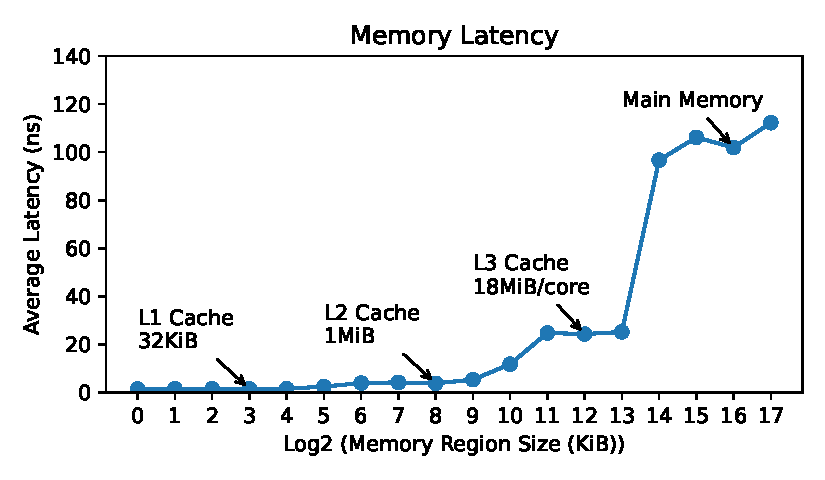
\includegraphics[width=0.98\linewidth]{sourcecode/memory/access_latency.pdf}
	\caption{\label{fig:access_lat} \textbf{RAM Access Latency}}
	%\vspace{-4mm}
\end{figure}
Figure~\ref{fig:access_lat} plots the RAM access latency result measured in our virtual machine (VM).
We can see that when we increase memory access region, the average access latency increase drastically
(from 1ns to more than 100ns). In each phase, we add a tag for current estimated access position from
L1, L2, L3, and to main memory. Experiment shows that L1 cache access latency is around 1.5ns,
L2 cache access latency is around 5ns, L3 cache access latency is around 25ns, and main memory access
latency is around 110ns.

\paragraph{Results analysis.}
For buffer sizes from 1 KiB to 32 KiB, the latency remains relatively low and consistent, suggesting these accesses are primarily served by the L1 cache. The L1 cache, being closest to the CPU and having the shortest access time, results in the lowest latency.

After a buffer size of 32 KiB, there is a noticeable increase in latency. This change is indicative of accesses beginning to spill over from the L1 cache to the L2 cache. The L2 cache, while larger than L1, has a longer access time, which results in increased latency.

As the buffer size further increases to 1024 KB and beyond, latency continues to rise. This trend is consistent with accesses reaching the L3 cache and eventually the main memory. The latency spike observed at buffer sizes of 16,384 KB and larger is particularly indicative of the transition to main memory, where access times are significantly higher than cache accesses. The main memory, being the furthest in the memory hierarchy from the CPU, exhibits the highest access latencies.

Overall, these results align with the expected behavior of our VM's memory hierarchies~\ref{table:sys-conf}. The initial low latency for smaller buffer sizes demonstrates the efficiency of CPU caches, while the increasing latency for larger sizes highlights the slower access times as data is fetched from progressively further memory layers.

\subsection{Memory Bandwidth}
\paragraph{Methodology.}
To measure the RAM bandwidth, our experiment was structured around two primary tests: reading from and writing to memory. The methodology focused on leveraging assembly language to perform these operations with minimal overhead and maximal efficiency. The assembly code was designed to bypass any compiler optimizations that could potentially skew the results.

For the read bandwidth test, a large memory block was sequentially accessed to read data, ensuring that the operation would span across the RAM's physical space. The time taken to complete this read operation was recorded. The write bandwidth test followed a similar approach, where a large memory block was sequentially written into, and the time for completion was recorded.

Both tests were conducted multiple times to account for any fluctuations in the system's state, ensuring that the results were repeatable and reliable. The average bandwidth was calculated by dividing the total size of the data transferred by the total time taken for the operation.

\paragraph{Experimental results.}
The results from the experiments are as follows:
%\begin{itemize}[leftmargin=*]
%	\item Read Bandwidth: 11.360022 GB/sec
%	\item Write Bandwidth: 7.637086 GB/sec
%\end{itemize}

\begin{table}[h]
	\centering
	\begin{tabular}{c|c|c}
		\hline
		\makecell{Type} & estimated & measured\\ \hline
        \textbf{Read Bandwidth} &  12.0 GB/s & 11.36 GB/s  \\ \hline
        \textbf{Write Bandwidth} & 12.0 GB/s & 7.64 GB/s  \\ \hline
	\end{tabular}
	\caption{\textbf{RAM Bandwidth}}
	\label{table:ram-band}
\end{table}

These results were obtained under controlled conditions to minimize interference from other system processes.

\paragraph{Results analysis.}
The read bandwidth of 11.360022 GB/sec signifies the efficient data retrieval capability of the system's RAM. This high rate of data transfer for reading operations indicates a well-performing memory subsystem, suitable for tasks that require rapid access to large volumes of data.

On the other hand, the write bandwidth, at 7.637086 GB/sec, while lower than the read bandwidth, still reflects a strong performance. The difference in read and write speeds can be attributed to the intrinsic design of memory technologies, where writing data typically involves more complex operations than reading.

The results align with expected behavior in our VM's memory architectures, where read operations are generally faster than write operations. The significant bandwidths recorded for both read and write operations demonstrate the capability of the system's memory to handle high-demand applications and processes.

Overall, the experiment successfully showcased the system's memory bandwidth, providing valuable insights into its performance characteristics in both reading and writing operations.

\subsection{Page Fault Service Time.}
\paragraph{Methodology.}
The methodology for measuring the page fault service time involved a three-step process tailored to ensure accurate measurement of the time taken to handle a page fault, specifically focusing on the scenario where data is fetched from the disk rather than from the system's cache.

First, a large file of 5GB was created and written with data. This size was chosen to ensure that it significantly exceeds the system's total memory of 904MB, thereby guaranteeing that not all data could be cached in memory. After writing the data to the file, \emph{fsync} was used to force the file's contents to be physically written to the disk, ensuring that subsequent file accesses would indeed involve disk reads.

Second, before measuring the page fault service time, the system's buffer and cache were cleared using Linux command-line (i.e., \emph{echo 3 > /proc/sys/vm/drop\_caches}). This step was crucial to ensure that the data would indeed have to be read from the disk, triggering page faults, rather than being served from the cached memory.

Third, the function designed to measure the page fault service time was executed. This function involved accessing the data from the previously created file, thereby triggering page faults. The time taken to service these faults was recorded, providing a measure of the average service time for each page fault.

\paragraph{Experimental results.}
The average page fault service time is shown as Table~\ref{table:ram-pagefault}.
This result represents the average time taken by the system to handle a single page fault when fetching data from the disk.

\begin{table}[h]
	\centering
	\begin{tabular}{c|c|c}
		\hline
		\makecell{Type} & estimated & measured\\ \hline
        \textbf{Pagefault} &  70-90$\mu$s & 27$\mu$s  \\ \hline
	\end{tabular}
	\caption{\textbf{Pagefault}}
	\label{table:ram-pagefault}
\end{table}

\paragraph{Results analysis.}
The average page fault service time of 0.026765 ms indicates the efficiency of the system's disk-based paging mechanism. Considering the limited total memory of 904MB~\ref{table:sys-conf} and the use of a 5GB file, the system was compelled to frequently access the disk to retrieve data not present in memory, leading to numerous page faults.

Dividing by the size of a page, it is much higher than accessing a byte from main memory as we measured before.
The relatively low page fault service time under these conditions suggests a reasonably swift disk access speed and an efficient page handling mechanism by the operating system. It is worth noting that page fault service times can be significantly influenced by various factors, including disk speed, the efficiency of the operating system's paging algorithms, and the overall system load.

In summary, the experiment effectively demonstrates the system's capability to handle page faults, providing a quantifiable measure of the time taken to retrieve data from the disk under conditions that simulate a memory-intensive workload. This insight is particularly valuable for understanding the system's performance in scenarios where the working set size exceeds the available physical memory.